\documentclass[12pt,a4paper]{article}
\usepackage{cmap}
\usepackage[utf8]{inputenc}
\usepackage{amsmath}
\usepackage{amsfonts}
\usepackage{amssymb}
\usepackage[left=1.5cm,right=1.5cm,top=1.75cm,bottom=1.75cm]{geometry}

\newcommand{\timelimit}{}

\usepackage{tikz}
\usetikzlibrary{automata, positioning, arrows}


\begin{document}
\pagestyle{empty}
\noindent

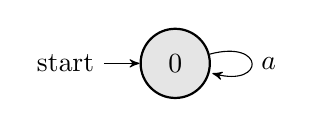
\begin{tikzpicture}[->, >=stealth', on grid, auto, node distance = 2.5cm, every state/.style={thick, fill=gray!20}]
\node[state, initial](0)at(-5.0, -0.0){0};

\path
(0)
    edge [loop right]node {$a$}(0)
;

\end{tikzpicture}
\end{document}

